% !TeX root = ../main.tex

\chapter{系统需求分析}

本章主要介绍数据湖分析系统的需求分析过程,主要包括系统概述、功能性
需求分析、非功能性需求分析三部分。针对公司目前面临的挑战和业务痛点,梳理业
务流程,确定项目需求。然后将需求划分为不同的功能,进行用例图展示,为后续的系统设计以及开发测试工作奠定基础。

\section{系统概述}

虽然数据湖在企业内部的需求很高,但开发人员使用的门槛较高,需要根据Apache Iceberg
官网的教程编写java程序来实现数据的入湖或者读取,这就对不太熟悉java的开发人员来说
不太友好,并且Iceberg后续的运维成本对于开发人员来说也比较高。因此开发了数据
湖分析系统,数据湖分析系统可以轻松完成T+0实时入湖,支持批流融合、秒级分析、事务语义、挖掘和探索数据价值等。

数据湖分析系统底层基于Apache Iceberg作为数据湖载体,开发框架使用Spring Boot,包含数
据源管理、元数据管理、数据入湖、数据探索、自动优化服务五大功能,其中自动优化服务是通过
内部调研发现,用户认为iceberg的运维成本较高,学习成本较大,所以设计了数据自动优化服务,帮助用户一键式优化。
并且数据湖分析系统还在Iceberg侧实现了小文件合并优化的功能,不但减少了小文件的数量增强了Iceberg的查询能力,而且还降低了用户的运维成本。

\section{系统功能性需求}

上一小节系统概述中,将数据湖分析系统划分为五大功能,在本节中将针对每一个功能进行详细分析。其总体的功能结构图如图\ref{fig:总体功能结构图}所示,
可以看到,数据自动优化服务是在元数据管理中实现的,包括小文件合并、历史快照清理、孤儿文件删除、数据生命周期管理等功能,会在后面进行详细的需求分析;
在数据源管理中,包括mysql数据源管理、tube数据源管理、kafka数据源管理、pulsar数据源管理的功能;
在元数据管理中,除了数据优化服务,还有表的增删改查、关联别处已创建的表、库的注册与查看等功能;
在数据入湖中,包括实时数据入湖、存量数据入湖、关系型数据入湖任务创建的功能;
在数据探索中,主要包括spark查询、presto查询、api方式查询、zeppelin查询的功能,其中,前三种查询方式会在内部的统一查询平台提供,
而zeppelin会内嵌在数据湖分析平台中供用户使用。

\begin{figure}[H]
  \centering
  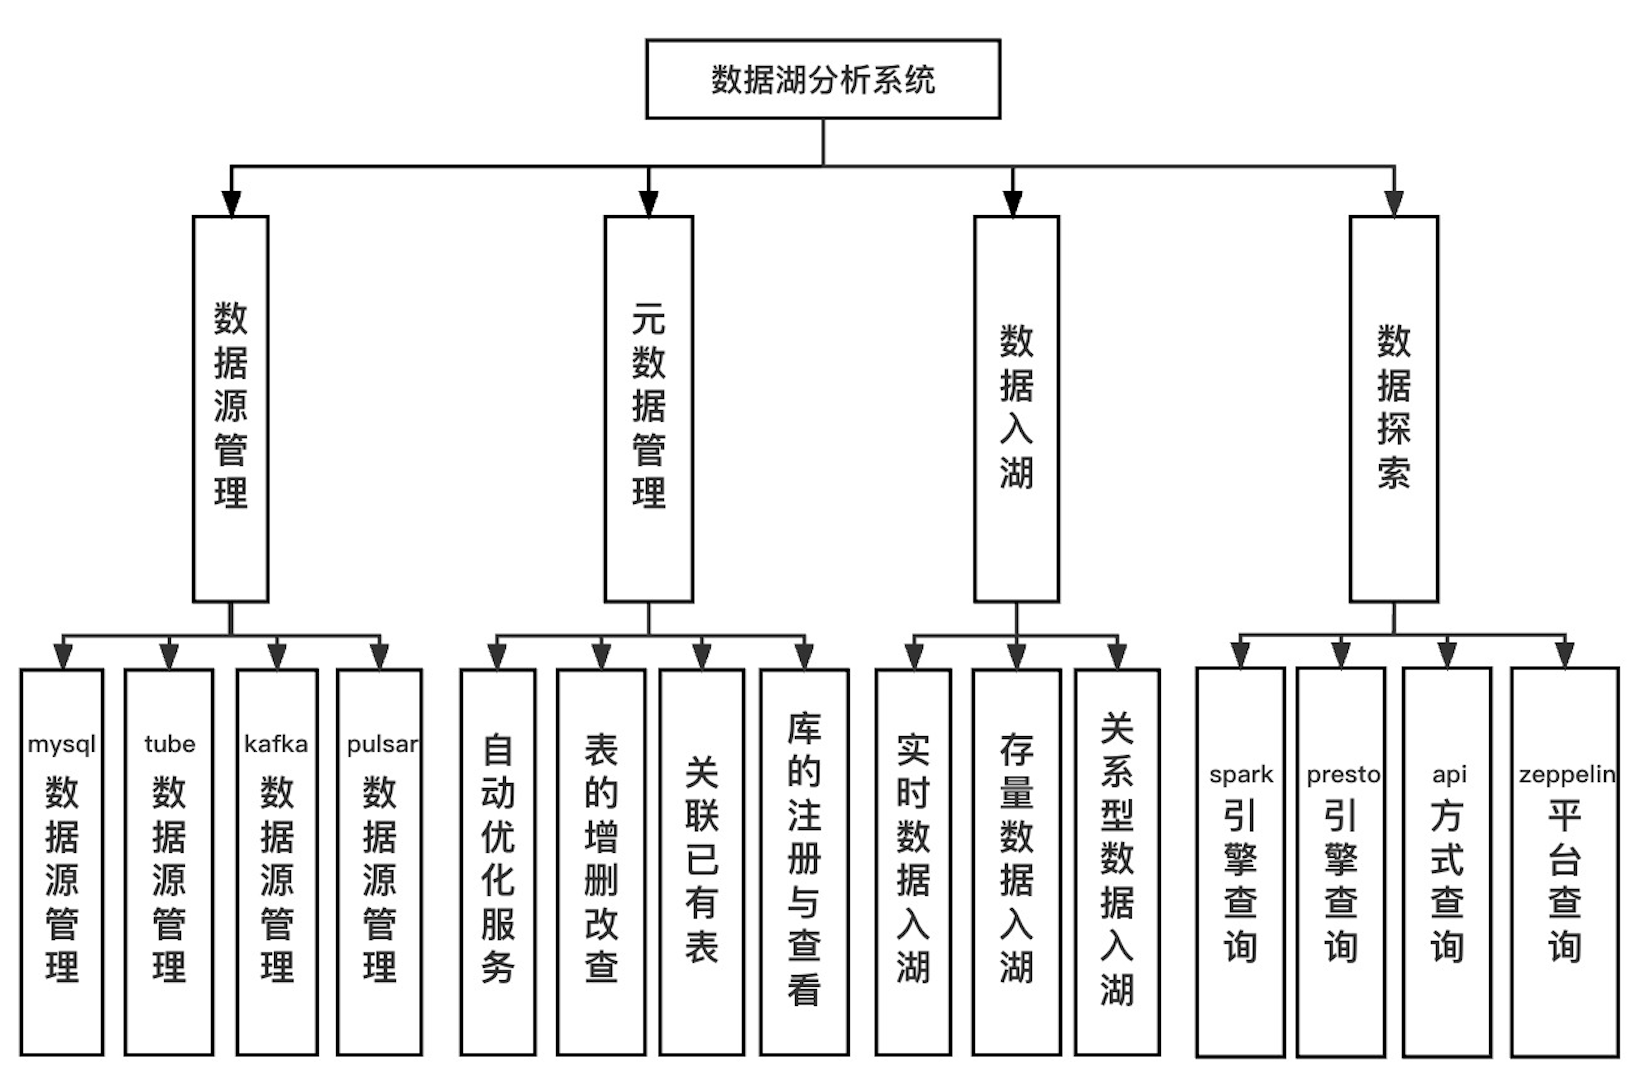
\includegraphics[width=1.0\textwidth]{总体功能结构图.png}
  \caption{总体功能结构图}
  \label{fig:总体功能结构图}
\end{figure}

\subsection{数据源管理功能}

数据源是入湖任务的前提要求,注册相应数据源,创建入湖任务时即可根据创建的数据源选择对应的源表。
数据源管理主要对数据源进行管理,其中关系型数据库支持Mysql,消息队列数据源支持Tube、Kafka、
Pulsar等数据源;支持数据源创建、查看、编辑、删除功能。数据源管理功能的需求用例图如图\ref{fig:数据源用例图}所示:

\begin{figure}[H]
  \centering
  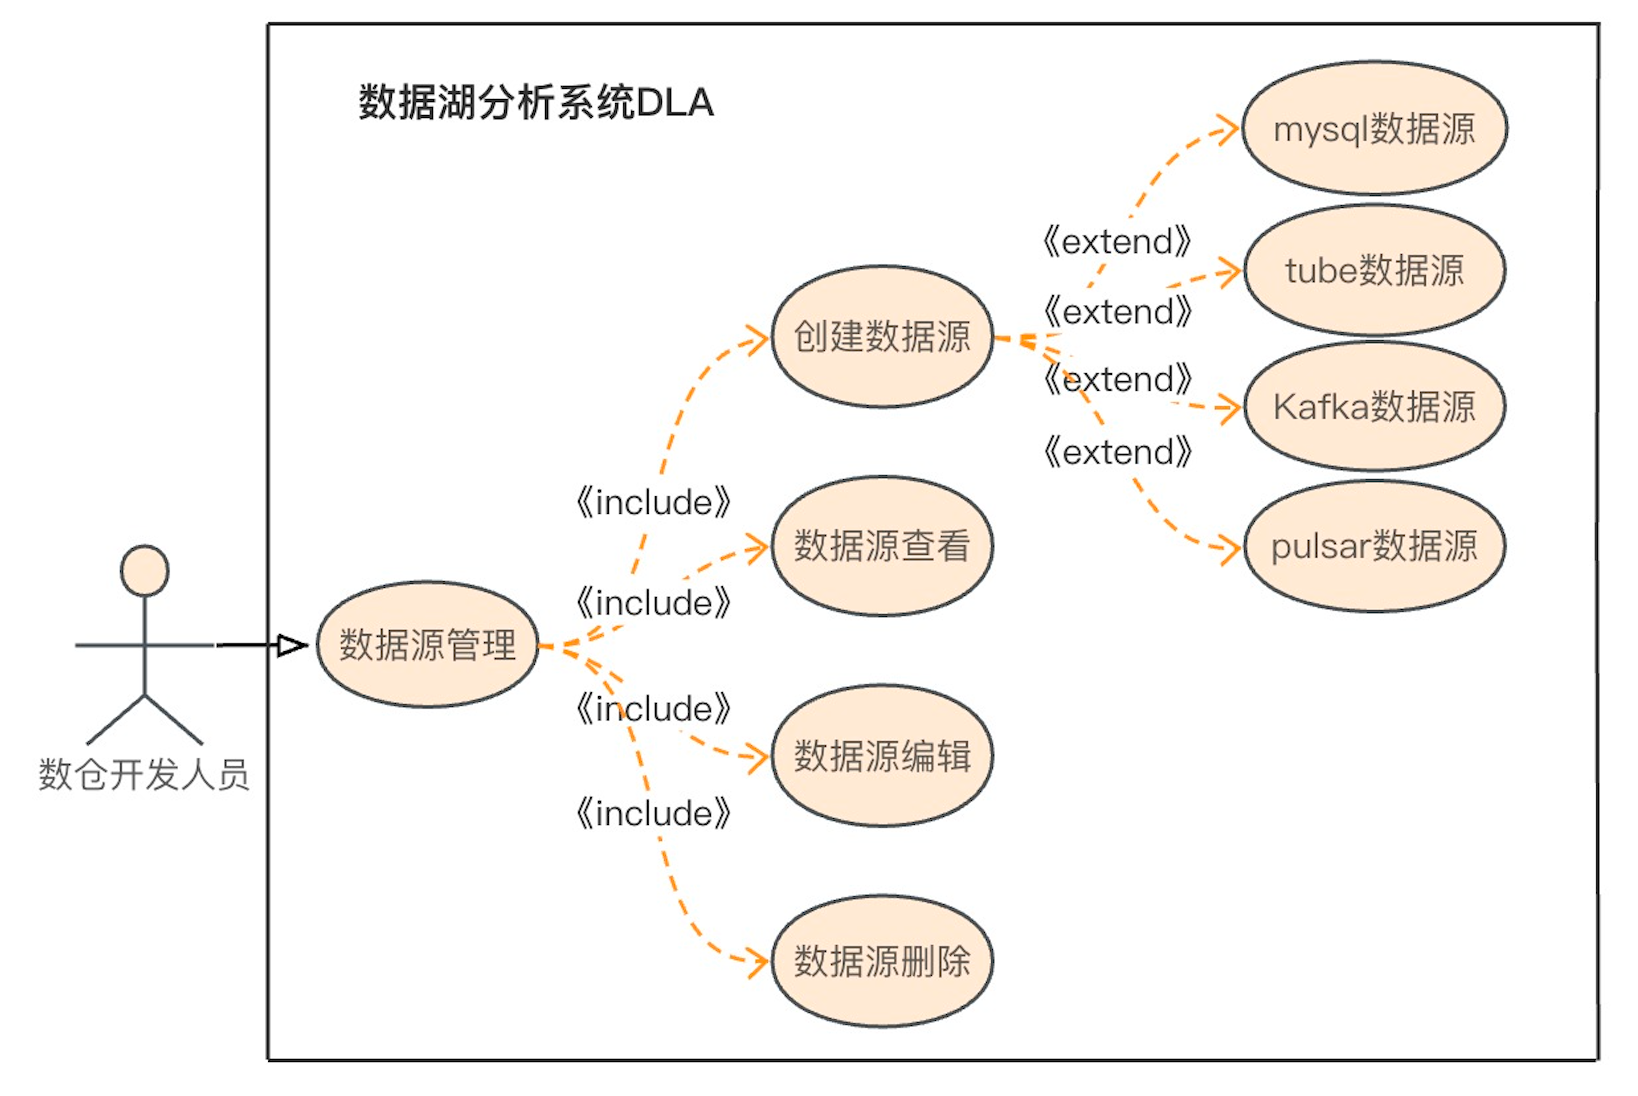
\includegraphics[width=0.85\textwidth]{数据源用例图.png}
  \caption{数据源管理功能用例图}
  \label{fig:数据源用例图}
\end{figure}

\subsection{元数据管理功能}

元数据是描述其他数据的数据,或用于提供有关资源信息的结构化数据。元数据是描述信息资源或数据等对象的数据,
它可以识别、评估和跟踪资源在使用过程中的变化\cite{15}。

这里的元数据是描述iceberg表的,iceberg表即目标表,是入湖任务的前提要求,
可以创建新表或者关联已有的表,在创建入湖任务时即可选择对应的目标表。元数据管
理主要对iceberg元数据进行管理,包含四个主要的功能,分别是数据自动优化、表的
操作、关联别处已创建的表、库的操作。其中数据优化功能会在后面进行详细介绍,表的操作包括iceberg
表的创建、查看、编辑、删除,关联别处已创建的表是关联在其它平台上已创建的iceberg表;
库操作包括注册数据库到数据湖和库的查看。
元数据管理功能的需求用例图如图\ref{fig:元数据用例图}所示:

\begin{figure}[H]
  \centering
  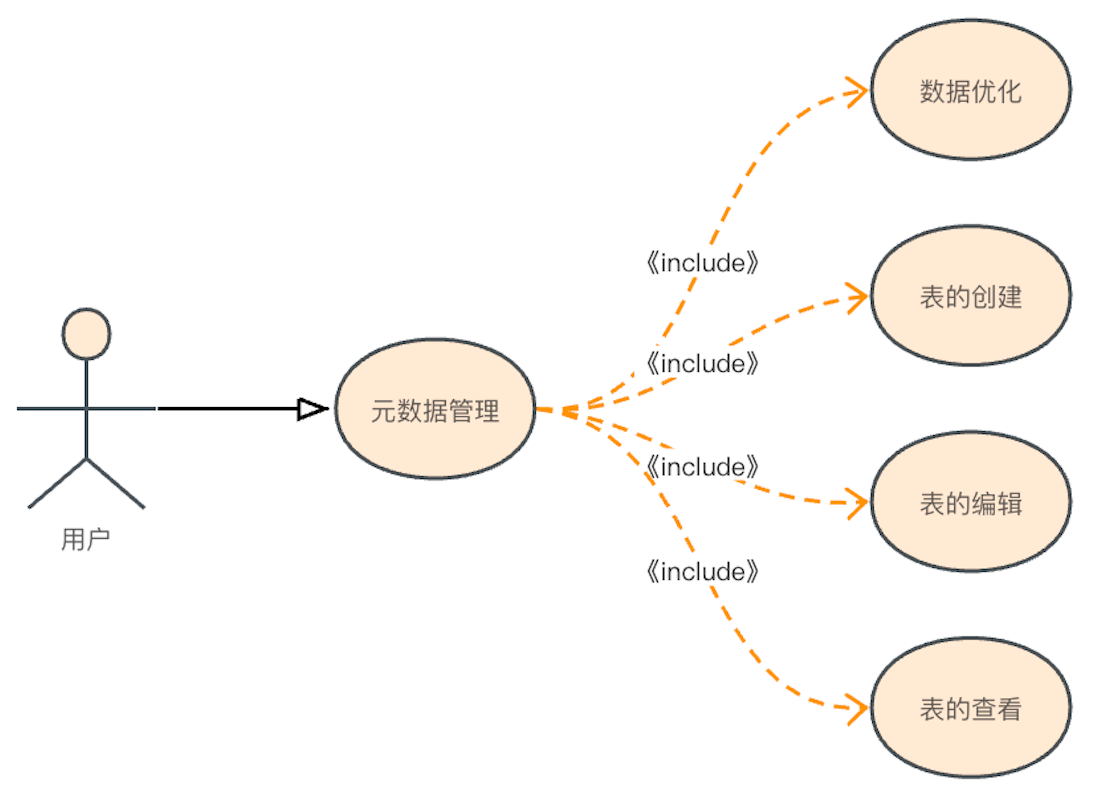
\includegraphics[width=0.80\textwidth]{元数据用例图.png}
  \caption{元数据管理功能用例图}
  \label{fig:元数据用例图}
\end{figure}

\subsection{数据入湖功能}

数据入湖功能是数据湖分析系统核心流程功能,目的是用户通过该功能将源数据表流程化入湖和查看
已申请入湖任务执行情况,目前支持的入湖类型为实时入湖(tube入湖、kafka入湖、pulsar入湖)
、存量入湖(data warehouse数据入湖)、关系型数据库入湖(mysql全量、增量入湖)。
其中实时入湖就是流形式的入湖,底层使用的flink来实现的;存量入湖就是批形式的入湖,底层使用的
spark来实现的;关系型数据入湖是指数据源是mysql,有全量、增量两种方式,全量就是只执行一次,
增量就是需要设置时间间隔、起始时间来定时更新。数据入湖功能的需求用例图如图\ref{fig:数据入湖用例图}所示:

\begin{figure}[H]
  \centering
  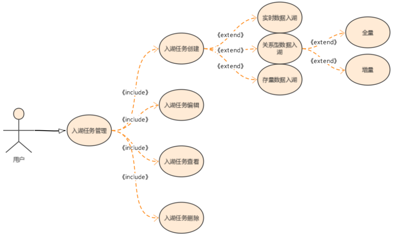
\includegraphics[width=0.80\textwidth]{数据入湖用例图.png}
  \caption{数据入湖功能用例图}
  \label{fig:数据入湖用例图}
\end{figure}

创建入湖任务总共需要五步:

(1)填写基础信息,根据入湖需要选择对应的入湖分类,填写必要的任务名;

(2)填写源表,实时入湖与关系型数据库入湖需要提前注册数据源,选择对应数据源表;

(3)填写目标表,所有入湖任务基本一致,支持推荐Schema功能,无需提前新建表,若目标表未创建,则任务创建时会自动的创建与源表对应的目标表,简化了创建目标表流程;

(4)查看映射预览,对源表及目标表schema映射展示,schema不一致无法进行下一步;

(5)填写参数及资源,对任务的资源进行配置。

\subsection{数据探索功能}

数据探索是数据入湖后,用户可以使用Spark、Presto、Zeppelin等引擎来进行查询分析数据,以实现数据的价值。
数据探索的用例图如图\ref{fig:数据探索用例图}所示:

\begin{figure}[H]
  \centering
  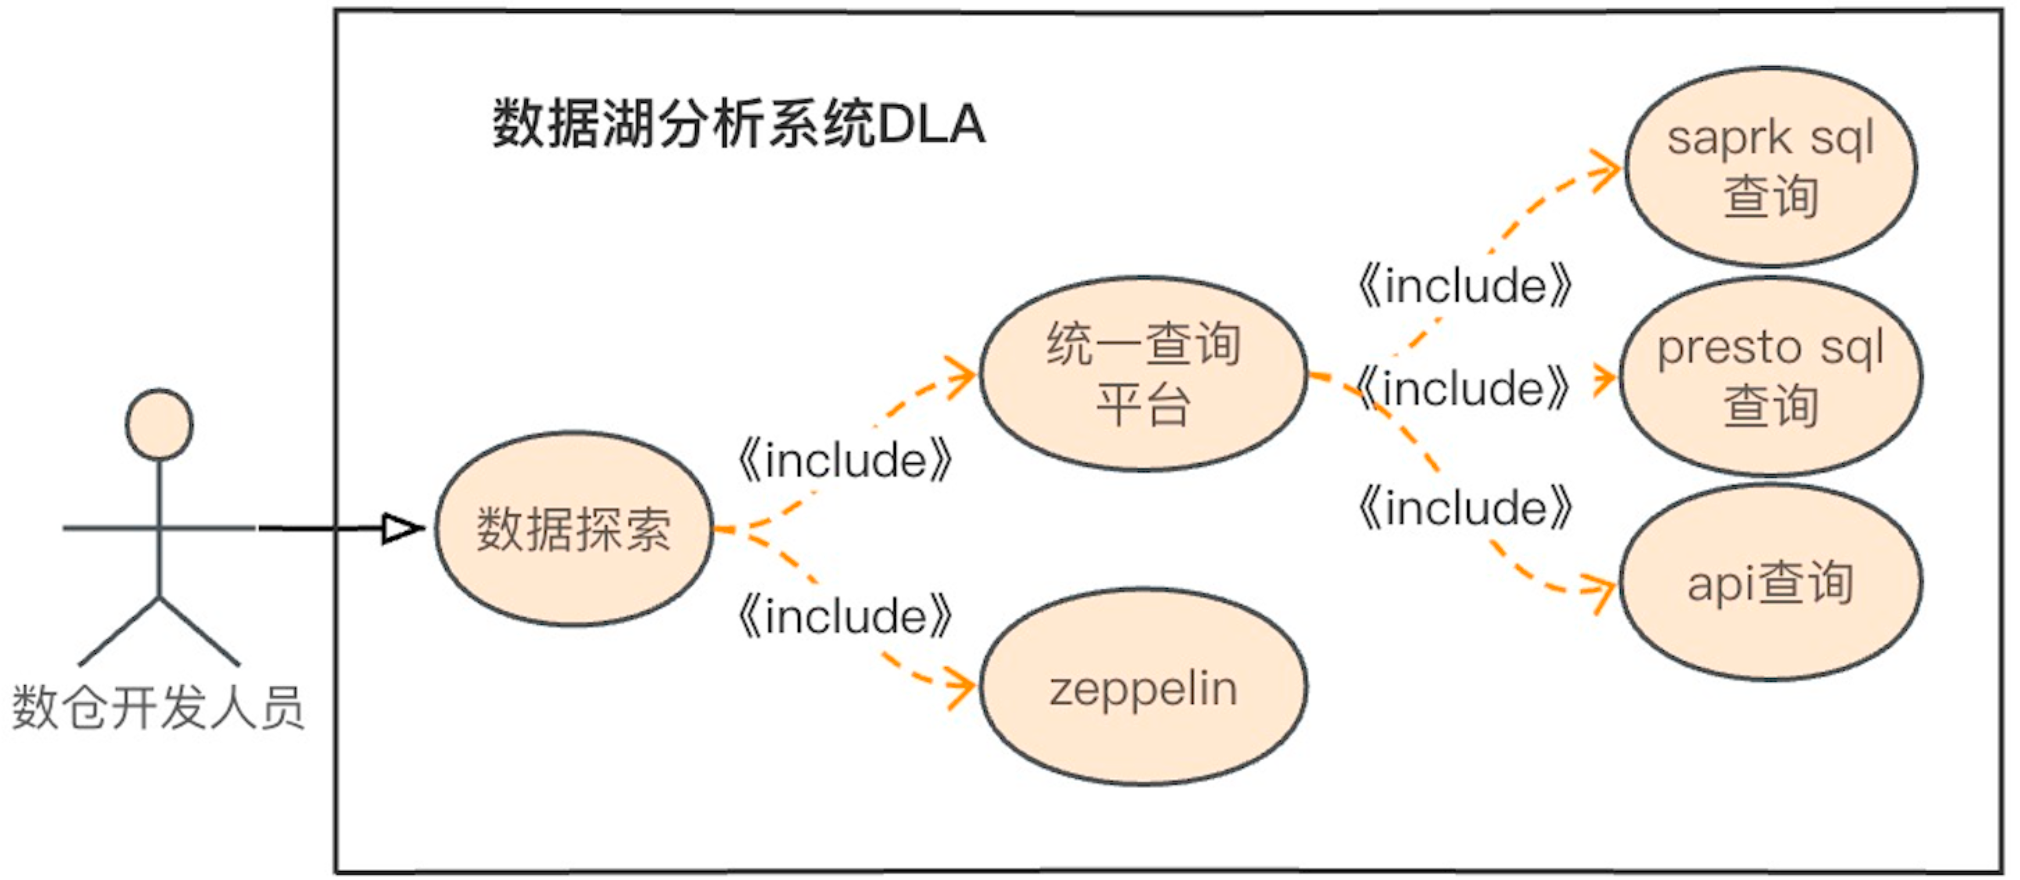
\includegraphics[width=0.80\textwidth]{数据探索用例图.png}
  \caption{数据探索功能用例图}
  \label{fig:数据探索用例图}
\end{figure}

在内部的统一查询平台上,用户可以选择Spark SQL或Presto SQL来完成数据的查询分析,其中,Presto的查询能力(select能力)突出,
可以实现秒级查询,但是Presto仅支持查询,其它的语句都不支持,相对的Spark的查询能力一般,
但是Spark支持的语句比较多,创建表、删除表、更新表、数据写入、数据删除、更新分区、表维护等
语句都是支持的。用户可以结合实际的情况灵活使用。

Zeppelin是一款数据科学和机器学习平台,旨在帮助数据科学家和分析师通过在notebook中
轻松地进行数据探索、可视化和建模。 Zeppelin支持多种数据源和语言
(如Python、R、Scala和SQL),并具有交互式的可视化和数据可视化功能。它还可以集成到
大数据生态系统中,如Apache Spark和Hadoop,以便处理大规模数据。 Zeppelin提供了一个
安全且易于管理的环境,可以帮助团队协作和追踪工作流程。最重要的是,Zeppelin是一个开源项目,
社区支持非常活跃,使其成为一款不断发展和改进的数据科学和机器学习平台\cite{34}。

\subsection{自动优化服务}

当前Iceberg运维有以下缺点:
用户需自行写java程序维护;
用户估计经验值,设定资源,资源浪费,或者不足导致失败;
若合并频率低,小文件多,则查询效率低,查询消耗资源多,合并频率高,可能导致重复合并,无法在适当的时间合并;
分区间数据不均衡时,无法按照分区合并,导致某些数据较少的分区被重复合并;
需持续观察任务执行情况,判断是何种原因导致失败,无告警。
为了解决这些缺点,DLA实现了数据自动优化服务,包括小文件合并、历史快照清理、孤儿文件删除、数据生命周期管理等服务。
其功能结构图如图\ref{fig:数据优化服务功能结构图}所示。自动优化服务有以下优点:
一键启动优化服务;
根据表的若干指标及历史执行情况判断所需资源;
合并恰如其时,根据写入的数据量判断合并的频次,查询速度稳定加快;
按照分区合并,仅合并需要合并的分区;
告警机制,专业运维及时处理。

\begin{figure}[H]
  \centering
  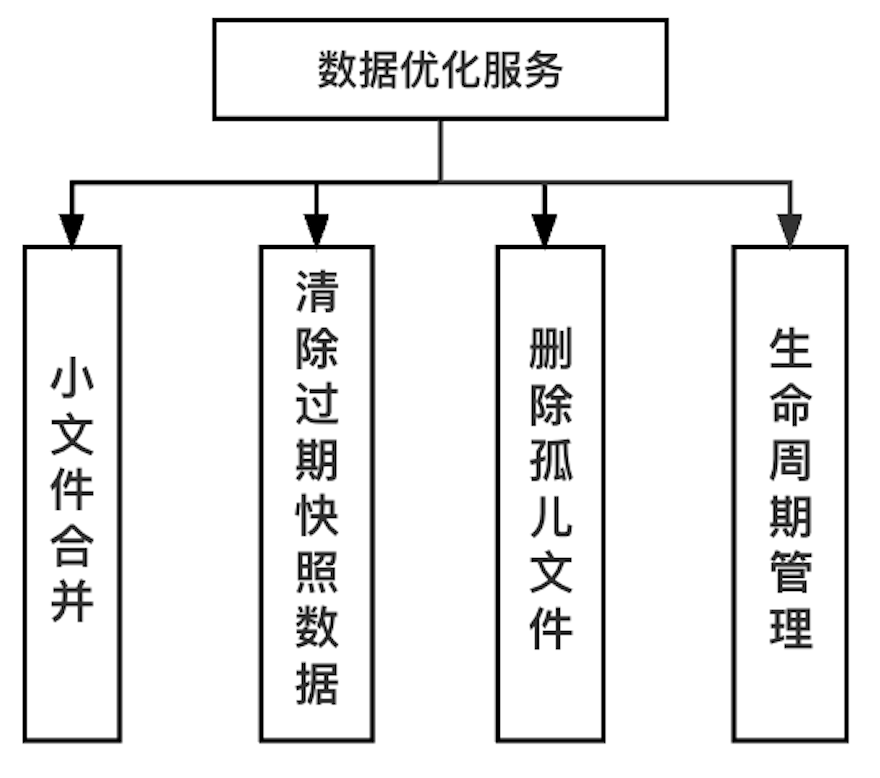
\includegraphics[width=0.5\textwidth]{数据优化服务功能结构图.png}
  \caption{数据优化服务功能结构图}
  \label{fig:数据优化服务功能结构图}
\end{figure}

\subsubsection{小文件合并}

由于hadoop一次写入,不可更改的特性,Iceberg写入会产生若干小文件,
尤其是在分区较多,并发写入较大的情况下,会加剧小文件数量,对HDFS NameNode造成压力,造成用户查询速度较慢\cite{35}。
将海量⼩⽂件进⾏合并为⼤⽂件,既可以提高查询效率降低数据存储成本,也能降低存储系统的元数据管理的压力。

由于原有的Iceberg小文件合并在实际应用中有着诸多的问题,比如合并不及时、浪费资源、
合并资源占用计算资源过多的问题。基于以上问题,重新设计了小文件合并规则。

关于小文件合并,Iceberg最初是通过在Flink Sink后接入Compaction Operator
的方式来进行在线的小文件合并,但随后发现在生产过程中存在很多的问题,最显著的就是
资源占用,因为其合并的任务逻辑属于Flink任务的一部分,需要占用Flink集群资源。
因此DLA通过数据自动优化服务来定期进行Iceberg表的compaction操作(生成saprk
任务来进行compaction)。然而定期调度存在对文件状态不确定,即不明确何时合并以及
是否小文件过多,这样就可能存在调度起了一个合并任务,但是任务执行只发现了2个小文件,
因为在这个定时的区间内只有2个小文件生成。如图\ref{fig:小文件合并定时任务调度}所示,
横坐标是合并任务序号,纵坐标是合并的小文件个数,可以看出定时调度任务执行的合并文件数非常不均衡。

\begin{figure}[H]
  \centering
  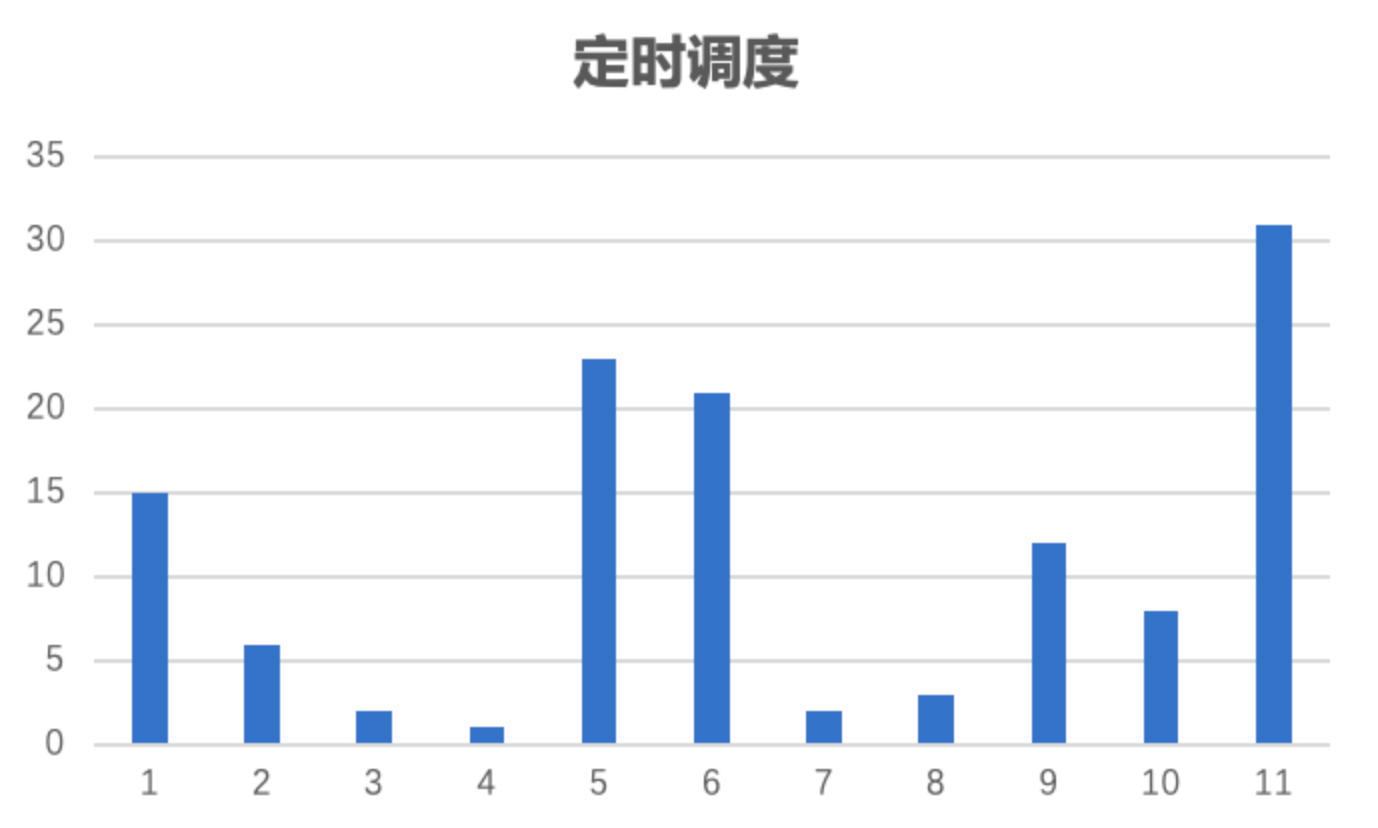
\includegraphics[width=0.85\textwidth]{小文件合并定时任务调度.png}
  \caption{定时任务调度合并文件数量}
  \label{fig:小文件合并定时任务调度}
\end{figure}

如图\ref{fig:小文件合并理想示意图}所示,在t2时刻将t1~t2期间产生的6个小文件进行了重写(即合并),
在t3时刻将t2~t3期间产生的2个小文件进行了合并,在t4时刻将t3~t4期间产生的7个小文件进行了合并,
而理想的状况是在t4时刻合并t2~t4期间生成的9个小文件,
该问题的核心点在于合并的任务无法知道当前的文件状态,因此需要一种计算规则来判断当前
一个区间内是否达到了发起合并任务的时刻,即需要计算出文件的状态,以作为合并任务调度的合并规则。

\begin{figure}[H]
  \centering
  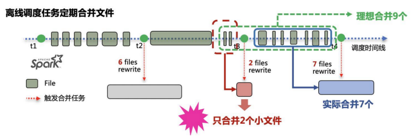
\includegraphics[width=1.0\textwidth]{小文件合并定时任务调度2.png}
  \caption{小文件合并理想示意图}
  \label{fig:小文件合并理想示意图}
\end{figure}

\subsubsection{历史快照清理}

由于Iceberg提供了time travel功能,所以元数据和数据文件会保留每条记录的多个版本快照(snapshot),
并且合并小文件时也会产生新的snapshot,但此时无用的小文件不会被立即删除。
如图\ref{fig:小文件合并场景}所示,DataFile A和DataFile B进行合并后,
生成了DataFile C以及新的元数据文件(Snapshot1和manifest1),但这里DataFile A和DataFile B已经是重复的数据了,
可以删除了。所以自动优化服务添加了历史快照清理,来清除这些不需要的数据。

\begin{figure}[H]
  \centering
  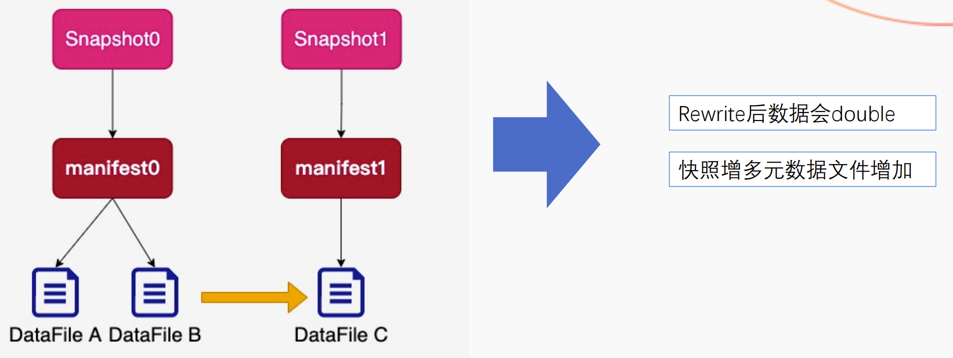
\includegraphics[width=1.0\textwidth]{小文件合并场景.png}
  \caption{小文件合并场景}
  \label{fig:小文件合并场景}
\end{figure}

\subsubsection{孤儿文件删除}

有的时候计算引擎执行任务失败,会产生一些不被引用的data和metadata files,
还有当rewrite失败或者commit失败时也会产生若干没有被引用的文件,这些文件都是孤儿文件,需要进行定期清理。
如图\ref{fig:孤儿文件产生场景}所示,在图中左侧,用户1对s1这条数据进行了更新操作,用户2对s1这条数据进行了删除操作
(在Iceberg中,更新或删除数据会生成对应的update或delete文件),并且在同一时刻进行了commit,这就会产生冲突,
这期间产生的update或delete文件就变成了孤儿文件;
在图中右侧,DataFile A和DataFile B进行了合并,但由于某些原因,合并失败了,
这期间产生的新的文件DataFile C和manifest1就变成了孤儿文件,需要进行清理。

\begin{figure}[H]
  \centering
  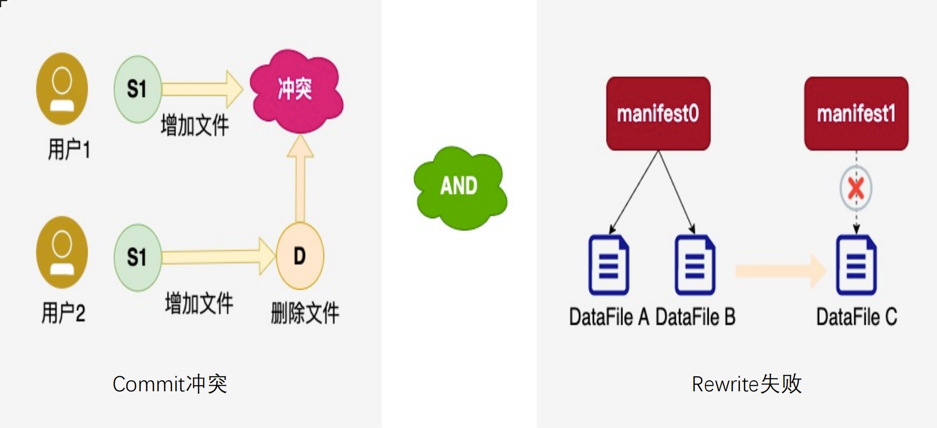
\includegraphics[width=1.0\textwidth]{孤儿文件产生场景.png}
  \caption{孤儿文件产生场景}
  \label{fig:孤儿文件产生场景}
\end{figure}

\subsubsection{数据生命周期管理}

为了更好的管理iceberg数据同时也为了节约用户成本,对数据的生命周期进行管理就显得尤为重要\cite{36}。
对数据进行生命周期管理,需要所创建的表中带有Date或TimeStamp类型的时间字段,并对此字段进行
操作删除过期数据。

\section{系统非功能性需求}

(1)性能需求。系统需要保证在高并发情况下能够快速响应用户请求,处理时间不超过2秒钟。

(2)端到端的数据展示低时延需求。在数据导入方面,系统要具有分钟级别的延迟,在数据查询方面,系统要具有
秒级分析的能力,这样整体端到端的数据展示时延就缩短到了分钟级。

(3)系统计算资源合理利用需求。系统要合理的根据任务基本情况进行资源申请,避免资源的浪费。

(4)系统安全性需求。系统需要采取多重安全措施来保护用户数据的安全性,如数据加密、用户身份验证等。

(5)可维护性需求。系统需要具有良好的可维护性,易于维护和升级,以确保系统的稳定性和可靠性。

(6)易用性需求。系统需要易于使用和学习,用户界面需要简洁明了,易于导航和操作。

(7)兼容性需求。系统需要与多种操作系统和浏览器兼容,以便用户可以在不同的设备上访问系统。

\section{本章小结}

在本章中首先对系统进行整体概述,明确项目目标以及应该具备的核心功能。
然后对数据源管理、元数据管理、数据入湖、数据探索、自动优化服务五方面详细
描述系统的功能性需求。最后从系统性能、端到端的数据展示低时延、计算资源合理利用、
安全性、兼容性等方面对系统的非功能性需求进行阐述。
